% SP09 mid-term report. Build from this folder:
%   pdflatex --disable-installer -interaction=nonstopmode midterm.tex   (run twice)
% Tables in tables/ and the trade-off figure are generated by scripts/validate_scipy.py;
% app screenshots by scripts/screenshots.py.
\documentclass[11pt,a4paper]{article}

\usepackage[T1]{fontenc}
\usepackage{lmodern}
\usepackage[margin=2.2cm]{geometry}
\usepackage{amsmath,amssymb}
\usepackage{graphicx}
\usepackage{xcolor}
\usepackage{array,tabularx}
\usepackage[shortlabels]{enumitem}
\usepackage{titlesec}
\usepackage{tikz}
\usetikzlibrary{arrows.meta,calc,positioning}
\usepackage[hidelinks]{hyperref}

% A captioned table that stays where it is written (the caption package is not installed).
\makeatletter
\newenvironment{fixedtable}{\par\noindent\begin{minipage}{\linewidth}\centering\def\@captype{table}}%
  {\end{minipage}\par\medskip}
\makeatother

\IfFileExists{author.tex}{\input{author}}{%
  \newcommand{\StudentName}{Student name}%
  \newcommand{\RollNo}{Roll number}%
  \newcommand{\Institute}{Institute}}

\hypersetup{pdftitle={SP09 Windowing Effects and Spectral Leakage Analyzer: Mid-Term Report},
  pdfauthor={\StudentName}}
\graphicspath{{figures/}}
\setlength{\parskip}{4pt}
\setlength{\parindent}{0pt}
\titlespacing*{\section}{0pt}{12pt}{4pt}
\titlespacing*{\subsection}{0pt}{8pt}{2pt}
\setlist{itemsep=1pt,topsep=2pt}
\renewcommand{\arraystretch}{1.15}
\newcolumntype{Y}{>{\raggedright\arraybackslash}X}
\newcommand{\bins}{\,\text{bins}}

\begin{document}

% ------------------------------------------------------------------ title block
\begin{center}
  {\small\textsc{EE4999 Signal Processing Project \textperiodcentered{} Mid-Term Report}}\\[8pt]
  {\LARGE\bfseries SP09: Windowing Effects and Spectral Leakage Analyzer}\\[6pt]
  {\large A web, Android and iOS app that compares common windows on finite sinusoids\\
  and quantifies main-lobe width and side-lobe levels}\\[10pt]
  \StudentName{} (\RollNo) \quad\textbar\quad Individual project\\[2pt]
  \Institute{} \quad\textbar\quad November 2026
\end{center}
\vspace{2pt}
\noindent\rule{\linewidth}{0.4pt}

\textbf{Summary.} The first half of the project is complete as a working web application
(version~0.5). It synthesises finite records of one or two sinusoids, applies one of seven
windows, and shows the resulting leakage in the time and frequency domains. It also measures
eight figures of merit for every window, including the main-lobe width (null-to-null,
$-3$\,dB, $-6$\,dB) and the peak side-lobe level. All signal processing (FFT, windows, metric
extraction) is our own code. It is checked by 23 automated tests and agrees with an
independent SciPy computation to within $2\times10^{-7}$\,dB and $10^{-8}$ bins. Validating it
also showed that several entries of the classic window table of Harris~\cite{harris} are
inaccurate. The second half adds more windows and analyses, and packages the app for Android
and iOS.

% ------------------------------------------------------------------ 1
\section{Problem Statement and Objectives}

Any measured signal is a \emph{finite} record. Taking the DFT of $N$ samples implicitly
multiplies the underlying signal by a window $w[n]$, so its spectrum is convolved with the
window's transform $W(e^{j\omega})$~\cite{oppenheim}. For a sinusoid this has three visible consequences:
\begin{itemize}
  \item \textbf{Spectral leakage:} the energy of each tone spreads into every DFT bin through
        the side lobes of $W$ and can bury weaker components.
  \item \textbf{Limited resolution:} the width of the main lobe sets how close two tones can be
        and still be told apart.
  \item \textbf{Scalloping:} a tone that falls between two bins is under-read by up to several dB.
\end{itemize}
Choosing a window trades main-lobe width against side-lobe level. Textbooks present this
trade-off as static tables and plots. There is no simple, cross-platform tool that shows the
effect on a sinusoid of the user's choosing and puts numbers on it. The project's objectives are:
\begin{enumerate}[label=\textbf{O\arabic*.}, leftmargin=2.6em]
  \item Generate finite records of sinusoids with user-chosen length $N$, sample rate $f_s$,
        frequency (on or off the DFT grid) and level.
  \item Provide the common windows: rectangular, Hann, Hamming, Blackman, Blackman--Harris,
        flat-top and Kaiser, in a form that can be extended later.
  \item Visualise leakage: the windowed record in time, and the DTFT together with the DFT
        samples in frequency, against a rectangular-window reference.
  \item Quantify each window: main-lobe width (null-to-null, $-3$\,dB, $-6$\,dB), peak
        side-lobe level, coherent gain, equivalent noise bandwidth, scalloping loss and
        worst-case processing loss. Side-lobe roll-off and resolution limits come later.
  \item Validate every reported number against an independent reference.
  \item Deliver the tool from one code base on the web, Android and iOS.
\end{enumerate}

% ------------------------------------------------------------------ 2
\section{Background: Windows and Their Figures of Merit}

For a record $x_w[n]=x[n]\,w[n]$, $n=0,\dots,N-1$, and a tone $x[n]=A\cos(\omega_0 n+\phi)$,
\begin{equation}
  X_w(e^{j\omega}) = \tfrac{A}{2}\left[e^{j\phi}\,W\!\left(e^{j(\omega-\omega_0)}\right)
                   + e^{-j\phi}\,W\!\left(e^{j(\omega+\omega_0)}\right)\right],
\end{equation}
and the $N$-point DFT samples this at $\omega_k = 2\pi k/N$. Frequencies below are expressed in
DFT bins, $\nu=\omega N/2\pi$. The windows implemented so far are the cosine-sum family and the
Kaiser window~\cite{kaiser},
\begin{equation}
  w[n]=\sum_{k=0}^{K}(-1)^k a_k\cos\frac{2\pi k n}{N},\qquad
  w_{\text{Kaiser}}[n]=\frac{I_0\!\left(\beta\sqrt{1-(2n/N-1)^2}\right)}{I_0(\beta)},
\end{equation}
with $a_k$ as in Table~\ref{tab:coeffs}. This is the \emph{periodic} (``DFT-even'') form used
for spectral analysis~\cite{harris}. The \emph{symmetric} form used in FIR design replaces $N$
by $N-1$ and is available as an option. Table~\ref{tab:defs} lists the figures of merit the
app measures.

\begin{table}[htbp]
  \centering\small
  \caption{Cosine-sum coefficients $a_0,\dots,a_K$ (the same values as SciPy).}
  \label{tab:coeffs}
  \begin{tabular}{ll}
    \hline
    Rectangular & $1$ \\
    Hann & $0.5,\ 0.5$ \\
    Hamming & $0.54,\ 0.46$ \\
    Blackman & $0.42,\ 0.5,\ 0.08$ \\
    Blackman--Harris (4-term) & $0.35875,\ 0.48829,\ 0.14128,\ 0.01168$ \\
    Flat-top (5-term) & $0.21557895,\ 0.41663158,\ 0.277263158,\ 0.083578947,\ 0.006947368$ \\
    \hline
  \end{tabular}
\end{table}

\begin{table}[htbp]
  \centering\small
  \caption{Figures of merit. $|W(\nu)|$ is the window's DTFT magnitude at $\nu$ bins and
  $\nu_0$ its first null.}
  \label{tab:defs}
  \begin{tabularx}{\linewidth}{lY}
    \hline
    Main-lobe width, null-to-null & $2\nu_0$ (bins) \\
    $-3$\,dB / $-6$\,dB width & $2\nu$ where $|W(\nu)|/|W(0)|$ falls to $10^{-3/20}$ / $10^{-6/20}$ \\
    Peak side-lobe level (PSL) & $\max_{\nu>\nu_0} 20\log_{10}|W(\nu)|/|W(0)|$ \\
    Coherent gain (CG) & $\frac{1}{N}\sum_n w[n]$ (amplitude gain for an on-bin tone) \\
    Equivalent noise bandwidth (ENBW) & $N\sum_n w^2[n]\,/\,\big(\sum_n w[n]\big)^2$ (bins) \\
    Scalloping loss (SL) & $-20\log_{10}|W(\tfrac12)|/|W(0)|$: worst under-reading, tone midway between bins \\
    Worst-case processing loss (WCPL) & $\mathrm{SL}+10\log_{10}\mathrm{ENBW}$: worst SNR loss for detecting a tone \\
    \hline
  \end{tabularx}
\end{table}

% ------------------------------------------------------------------ 3
\section{Approach and Methodology}

\subsection{Architecture}
The app is a client-side web application written in TypeScript (Figure~\ref{fig:arch}). The
user's settings drive two paths. The \emph{signal path} synthesises the record, applies the
window, zero-pads and transforms it, and plots it. The \emph{metrics path} measures the
selected windows. There is no server: every computation runs on the user's device, which is
also what makes offline mobile builds straightforward.

\begin{figure}[htbp]
  \centering
  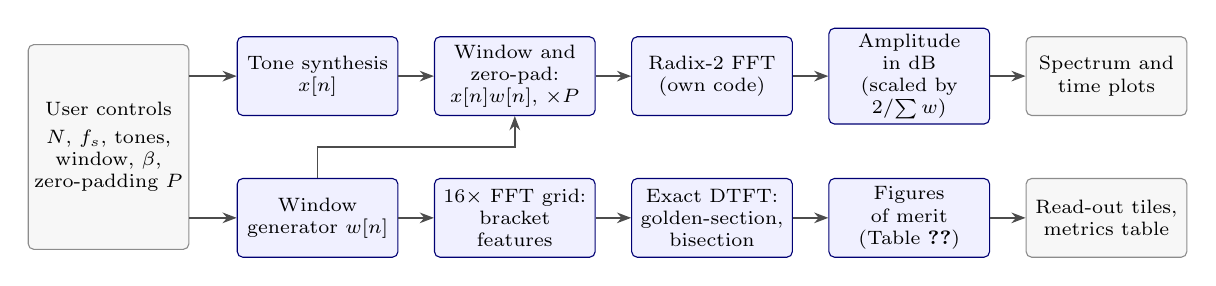
\begin{tikzpicture}[
      node distance=4.5mm and 4.5mm,
      box/.style={draw=black!45, rounded corners=2pt, fill=black!3, align=center,
                  font=\scriptsize, text width=19mm, minimum height=10mm, inner sep=2pt},
      dsp/.style={box, fill=blue!6, draw=blue!45!black},
      arr/.style={-{Stealth[length=1.8mm]}, semithick, draw=black!70}]
    \node[box, minimum height=26mm] (ui) {User controls\\[2pt] $N$, $f_s$, tones,\\window, $\beta$,\\zero-padding $P$};
    \node[dsp, right=6mm of ui, yshift=9mm] (gen) {Tone synthesis\\$x[n]$};
    \node[dsp, right=of gen] (mul) {Window and\\zero-pad: $x[n]w[n]$, $\times P$};
    \node[dsp, right=of mul] (fft) {Radix-2 FFT\\(own code)};
    \node[dsp, right=of fft] (db) {Amplitude in dB\\(scaled by $2/\!\sum w$)};
    \node[box, right=of db] (plots) {Spectrum and\\time plots};
    \node[dsp, right=6mm of ui, yshift=-9mm] (win) {Window\\generator $w[n]$};
    \node[dsp, right=of win] (grid) {16$\times$ FFT grid:\\bracket features};
    \node[dsp, right=of grid] (refine) {Exact DTFT:\\golden-section,\\bisection};
    \node[dsp, right=of refine] (fom) {Figures of merit\\(Table~\ref{tab:defs})};
    \node[box, right=of fom] (tab) {Read-out tiles,\\metrics table};
    \draw[arr] (ui.east |- gen) -- (gen);
    \draw[arr] (ui.east |- win) -- (win);
    \draw[arr] (gen) -- (mul);
    \draw[arr] (mul) -- (fft);
    \draw[arr] (fft) -- (db);
    \draw[arr] (db) -- (plots);
    \draw[arr] (win) -- (grid);
    \draw[arr] (grid) -- (refine);
    \draw[arr] (refine) -- (fom);
    \draw[arr] (fom) -- (tab);
    \coordinate (gap) at ($(gen.south)!0.5!(win.north)$);
    \draw[arr] (win.north) |- (gap -| mul.south) -- (mul.south);
  \end{tikzpicture}
  \caption{Processing architecture. Shaded blocks are the signal-processing modules written for
  this project (\texttt{src/dsp}); the rest is user interface.}
  \label{fig:arch}
\end{figure}

\subsection{Algorithms}
\begin{itemize}
  \item \textbf{FFT.} Iterative radix-2 Cooley--Tukey with a twiddle table computed directly
        (no recurrence, so it does not drift at large sizes). It agrees with a direct DFT to $10^{-9}$.
  \item \textbf{Spectrum display.} The windowed record is zero-padded by
        $P\in\{1,2,4,8,16\}$, which samples the DTFT $P$ times per bin. Every $P$-th point is
        exactly an $N$-point DFT bin and is drawn as a dot over the continuous DTFT. Scaling by
        $2/\sum w$ makes an on-bin tone of amplitude $A$ read $20\log_{10}A$, so scalloping
        shows up directly as an amplitude error.
  \item \textbf{Metric extraction.} (i)~Sample $|W|$ on a 16$\times$ oversampled FFT grid.
        (ii)~Take the first null to be the first local minimum below $-20$\,dB, so the pass-band
        ripple of a flat-top window cannot pass for a null. Refine it by golden-section search
        on the exact DTFT $W(\nu)=\sum_n w[n]e^{-j2\pi\nu n/N}$. (iii)~Find the $-3$/$-6$\,dB
        points by bisection on the exact DTFT inside the main lobe. (iv)~The PSL is the largest
        grid value beyond the first null, refined by golden-section search. (v)~CG and ENBW come
        from the samples, and SL from the exact DTFT at $\nu=\tfrac12$. The results therefore do
        not depend on the FFT grid.
\end{itemize}

\subsection{Validation strategy}
\begin{enumerate}[(a)]
  \item \textbf{Unit tests} (Vitest, 17 tests):
    \begin{itemize}
      \item FFT against a direct DFT, and window identities (symmetry; periodic = symmetric of
            length $N{+}1$ minus its last sample; Kaiser with $\beta=0$ is rectangular);
      \item metrics against closed forms: exact CG and ENBW; nulls at $K{+}1$ bins; large-$N$
            sinc-sum expressions for scalloping loss and widths; Kaiser half-width
            $\sqrt{1+(\beta/\pi)^2}$;
      \item peak side-lobe levels against published values.
    \end{itemize}
    Six DOM tests check the user-interface wiring.
  \item \textbf{Independent cross-check}: a Python script recomputes every metric using SciPy's
        windows~\cite{scipy} and a brute-force $2^{21}$-point FFT. This is a different algorithm
        from the app's, and the script fails if any metric differs by more than its tolerance.
  \item \textbf{Literature comparison} with Table~I of Harris~\cite{harris}.
\end{enumerate}

\subsection{Cross-platform plan and tools}
The interface is a responsive web app that already adapts to phone screens (Figure~\ref{fig:phone}).
The planned route to mobile is:
\begin{itemize}
  \item an installable Progressive Web App that works offline;
  \item a Capacitor wrapper producing an Android APK and an iOS build. The iOS build needs
        macOS and Xcode; if no Mac is available, iOS users install the PWA instead.
\end{itemize}
Tools used: TypeScript, Vite, uPlot (charts), Vitest and happy-dom (tests), Python with NumPy,
SciPy and Matplotlib (validation and figures), Playwright (screenshots), and Git/GitHub for
version control.

% ------------------------------------------------------------------ 4
\section{Work Completed and Preliminary Results}

\subsection{Implementation status}
Table~\ref{tab:status} lists what the mid-term build contains and what is planned for the
second half.

\begin{fixedtable}
  \small
  \caption{Feature status at mid-term.}
  \label{tab:status}
  \begin{tabularx}{\linewidth}{Yl}
    \hline
    Tone generator: one or two tones; $N=32$--$1024$; $f_s$; level; on- or off-grid frequency & Done \\
    Window library: 7 windows, periodic/symmetric definitions, adjustable Kaiser $\beta$ & Done \\
    Radix-2 FFT, zero-padded spectrum with the DFT bins overlaid, time-domain view & Done \\
    Eight figures of merit, measured on the exact DTFT & Done \\
    Leakage Explorer and Window Comparison views; responsive phone/tablet layout & Done \\
    23 automated tests; SciPy cross-check script; literature comparison & Done \\
    More windows (Bartlett, Tukey, Gaussian, Nuttall~\cite{nuttall}, Dolph--Chebyshev) & Planned \\
    Side-lobe roll-off; two-tone resolution and detectability analyser & Planned \\
    In-app trade-off charts, CSV/PNG export, shareable settings, dark mode & Planned \\
    PWA (offline), Android and iOS builds, public deployment & Planned \\
    \hline
  \end{tabularx}
\end{fixedtable}

\subsection{Leakage Explorer}
Figure~\ref{fig:leak} shows the main view. Figure~\ref{fig:spectra} isolates leakage,
scalloping and masking ($N=64$, $P=8$).
\begin{itemize}
  \item \textbf{On-bin tone} (10.00 bins, Figure~\ref{fig:spectra}a): apart from the tone's own bin, every DFT sample
        falls on a null of the rectangular kernel, so the DFT shows a single line. Those samples
        are exact zeros and are pinned to the bottom of the plot.
  \item \textbf{Same tone at 10.50 bins} (Figure~\ref{fig:spectra}b): every bin is non-zero, the far skirt decays slowly
        (only $-6$\,dB per octave), and the strongest bin reads $-3.79$\,dB instead of 0\,dB.
        That is the 3.92\,dB rectangular scalloping loss, slightly offset by leakage from the
        negative-frequency image.
  \item \textbf{Leakage hiding a weak tone} (Figure~\ref{fig:spectra}c): a second tone 60\,dB
        weaker sits 5.5 bins away. Rectangular leakage at that frequency is about $-25$\,dB, so
        the tone is invisible. With the Blackman--Harris window its side lobes are near
        $-92$\,dB and the weak tone stands out clearly. The main tone's strongest bin now reads
        $-0.83$\,dB, the Blackman--Harris scalloping loss.
\end{itemize}

\begin{figure}[htbp]
  \centering
  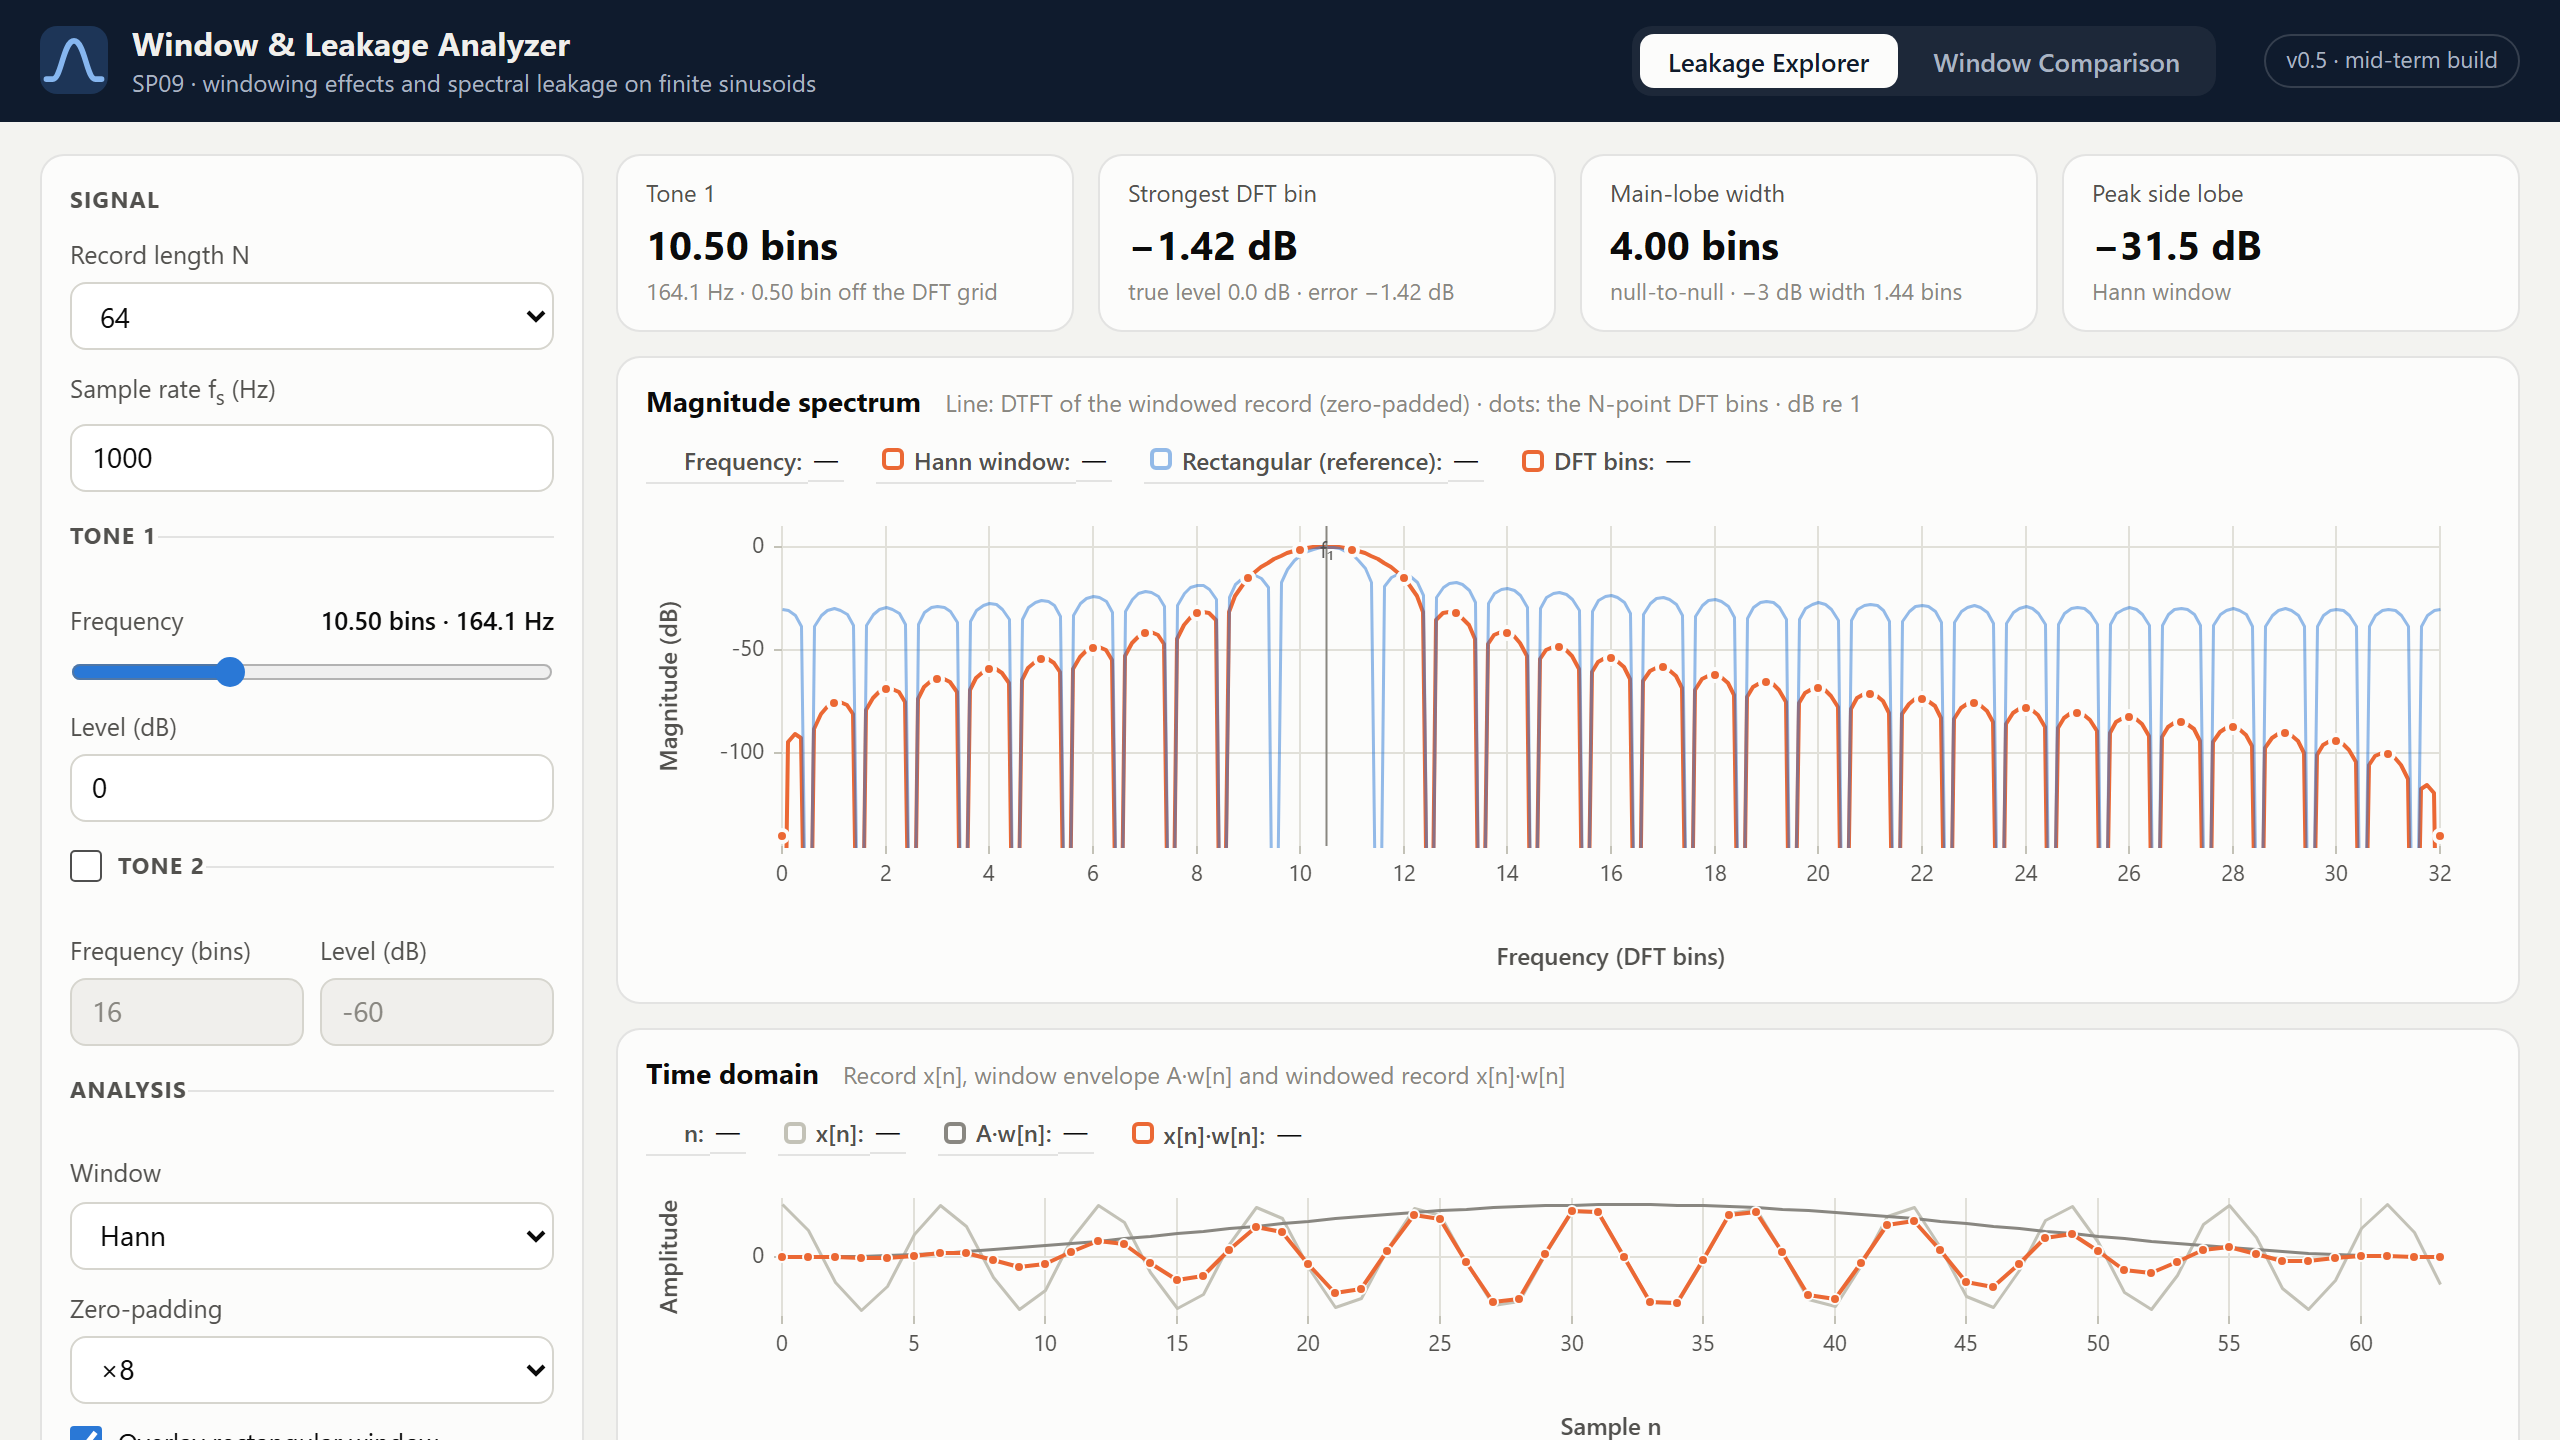
\includegraphics[width=\linewidth]{app_leakage.png}
  \caption{Leakage Explorer: controls (left), read-outs (top), spectrum with the DFT bins as dots,
  and time-domain view. Hann window, tone at 10.5 bins, rectangular reference in light blue.}
  \label{fig:leak}
\end{figure}

\begin{figure}[htbp]
  \centering
  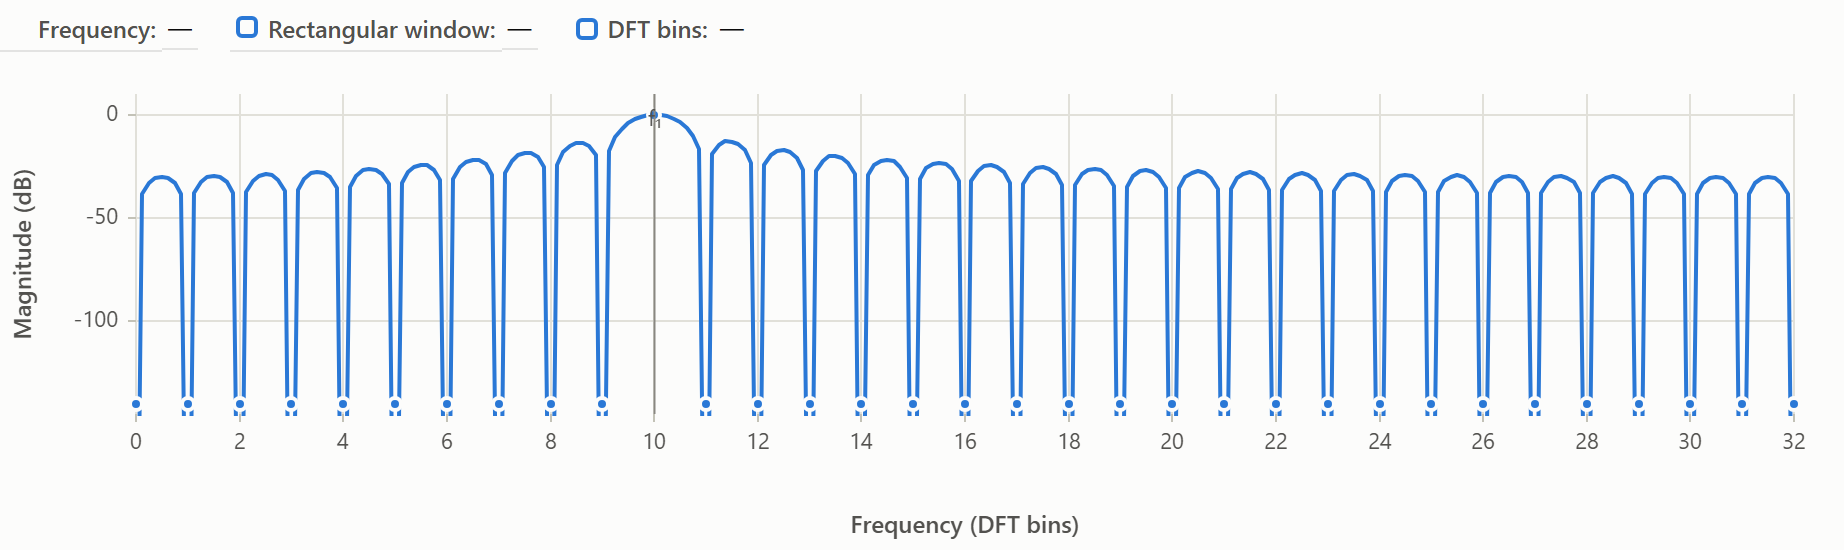
\includegraphics[width=0.95\linewidth]{spec_onbin.png}\\[-1pt]
  {\small (a) Rectangular window, tone on bin 10.00: the DFT samples (dots) fall on the kernel's
  nulls, so no leakage is visible.}\\[8pt]
  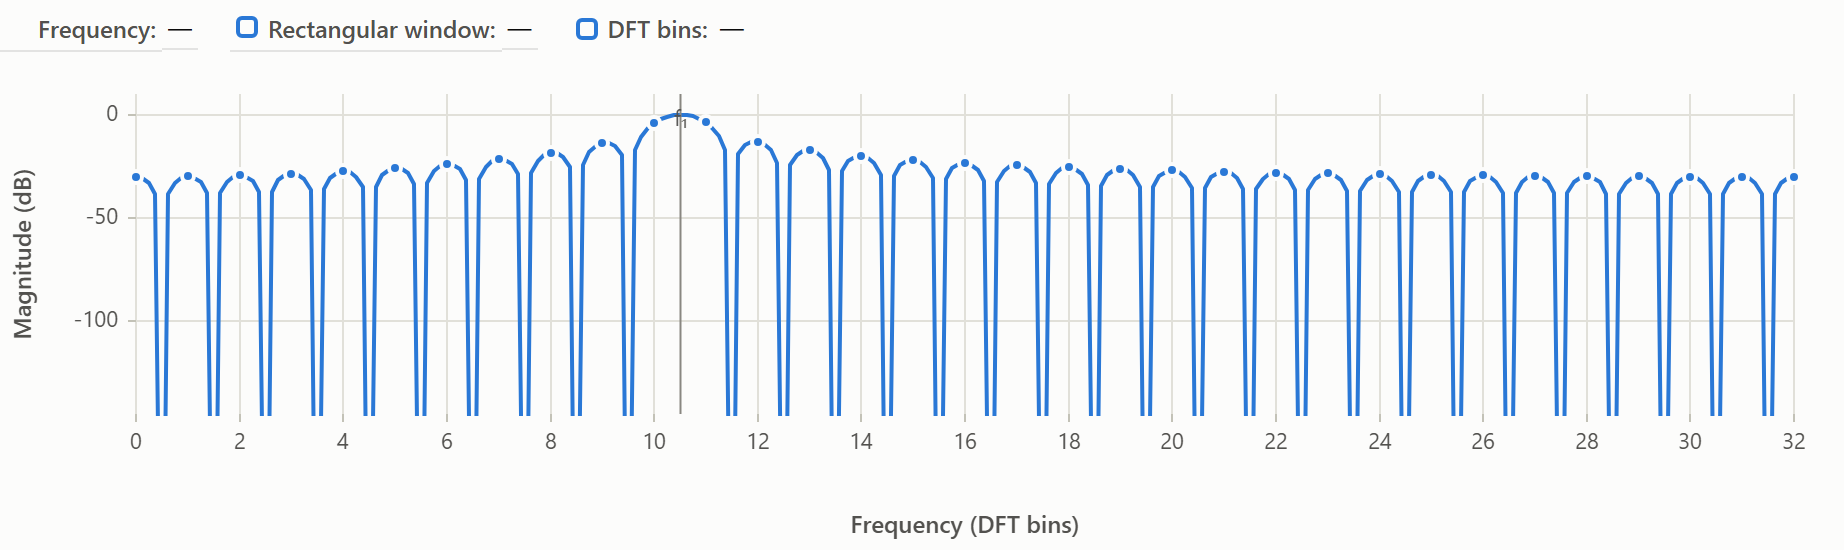
\includegraphics[width=0.95\linewidth]{spec_halfbin.png}\\[-1pt]
  {\small (b) The same tone at 10.50 bins: every bin leaks, and the strongest bin under-reads by
  3.8\,dB.}\\[8pt]
  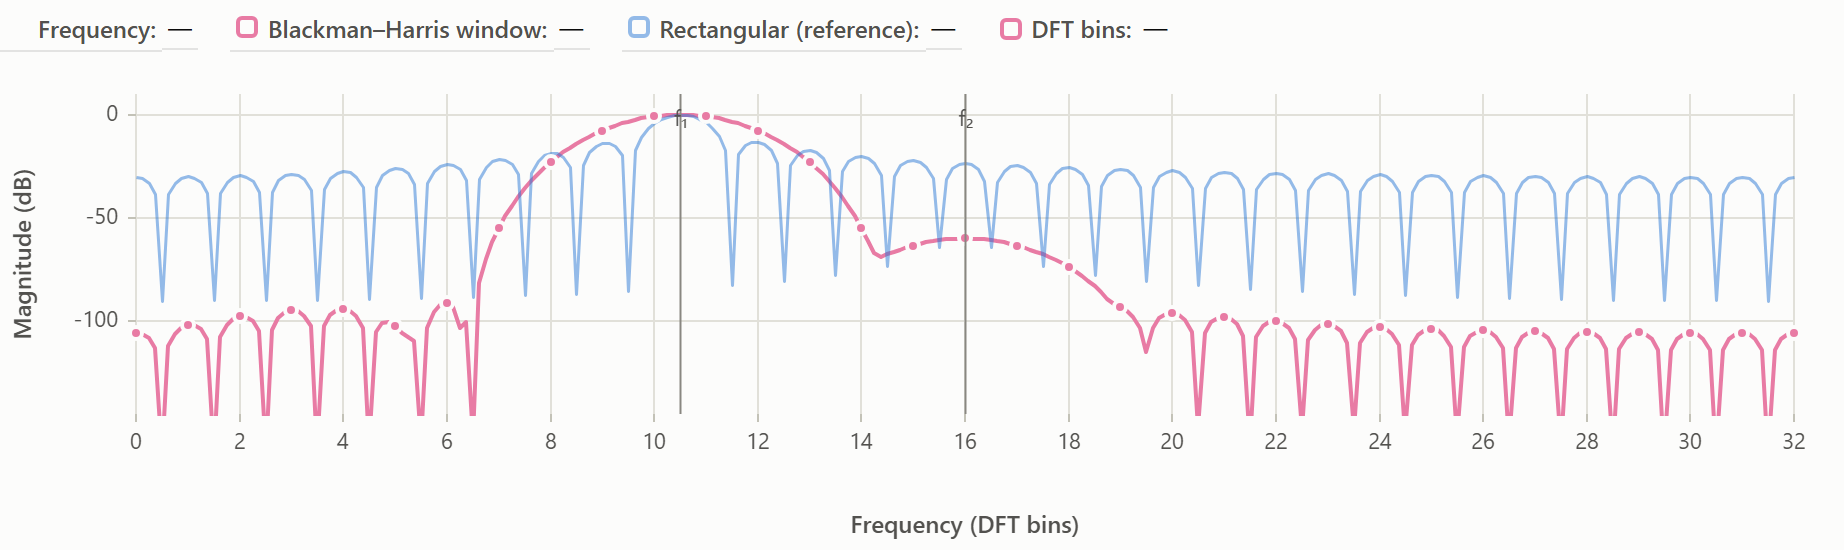
\includegraphics[width=0.95\linewidth]{spec_twotone.png}\\[-1pt]
  {\small (c) A $-60$\,dB tone added at 16 bins: buried under rectangular leakage (light blue),
  clearly visible with Blackman--Harris (pink).}
  \caption{Leakage, scalloping and masking in the Leakage Explorer ($N=64$, zero-padding
  $\times8$). Lines are the zero-padded DTFT; dots are the $N$-point DFT bins.}
  \label{fig:spectra}
\end{figure}

\subsection{Window Comparison and measured figures of merit}
The comparison view (Figure~\ref{fig:compare}) overlays the normalised responses and the window
shapes, and tabulates the figures of merit with the best value in each column highlighted.
Table~\ref{tab:metrics} lists the values measured by the app at $N=256$.
\begin{itemize}
  \item The rectangular window has the narrowest main lobe (0.88 bins at $-3$\,dB) but the
        worst side lobes ($-13.3$\,dB).
  \item Blackman--Harris reaches $-92.0$\,dB at 2.1 times that width.
  \item Flat-top reads amplitude almost exactly (0.01\,dB scalloping) at the cost of a main
        lobe 3.7 bins wide at $-3$\,dB.
  \item The Kaiser window covers the trade-off continuously (Figure~\ref{fig:tradeoff}). At
        $\beta=8.6$ it is as wide as Blackman (1.63 vs 1.64 bins) with side lobes 5\,dB lower
        ($-63.3$ vs $-58.1$\,dB).
  \item Hamming lies below the Kaiser curve: $-42.7$\,dB at 1.30 bins, where a Kaiser window
        of the same width reaches only about $-37$\,dB. This is because its two coefficients
        are tuned to cancel the first side lobe.
\end{itemize}

\begin{figure}[htbp]
  \centering
  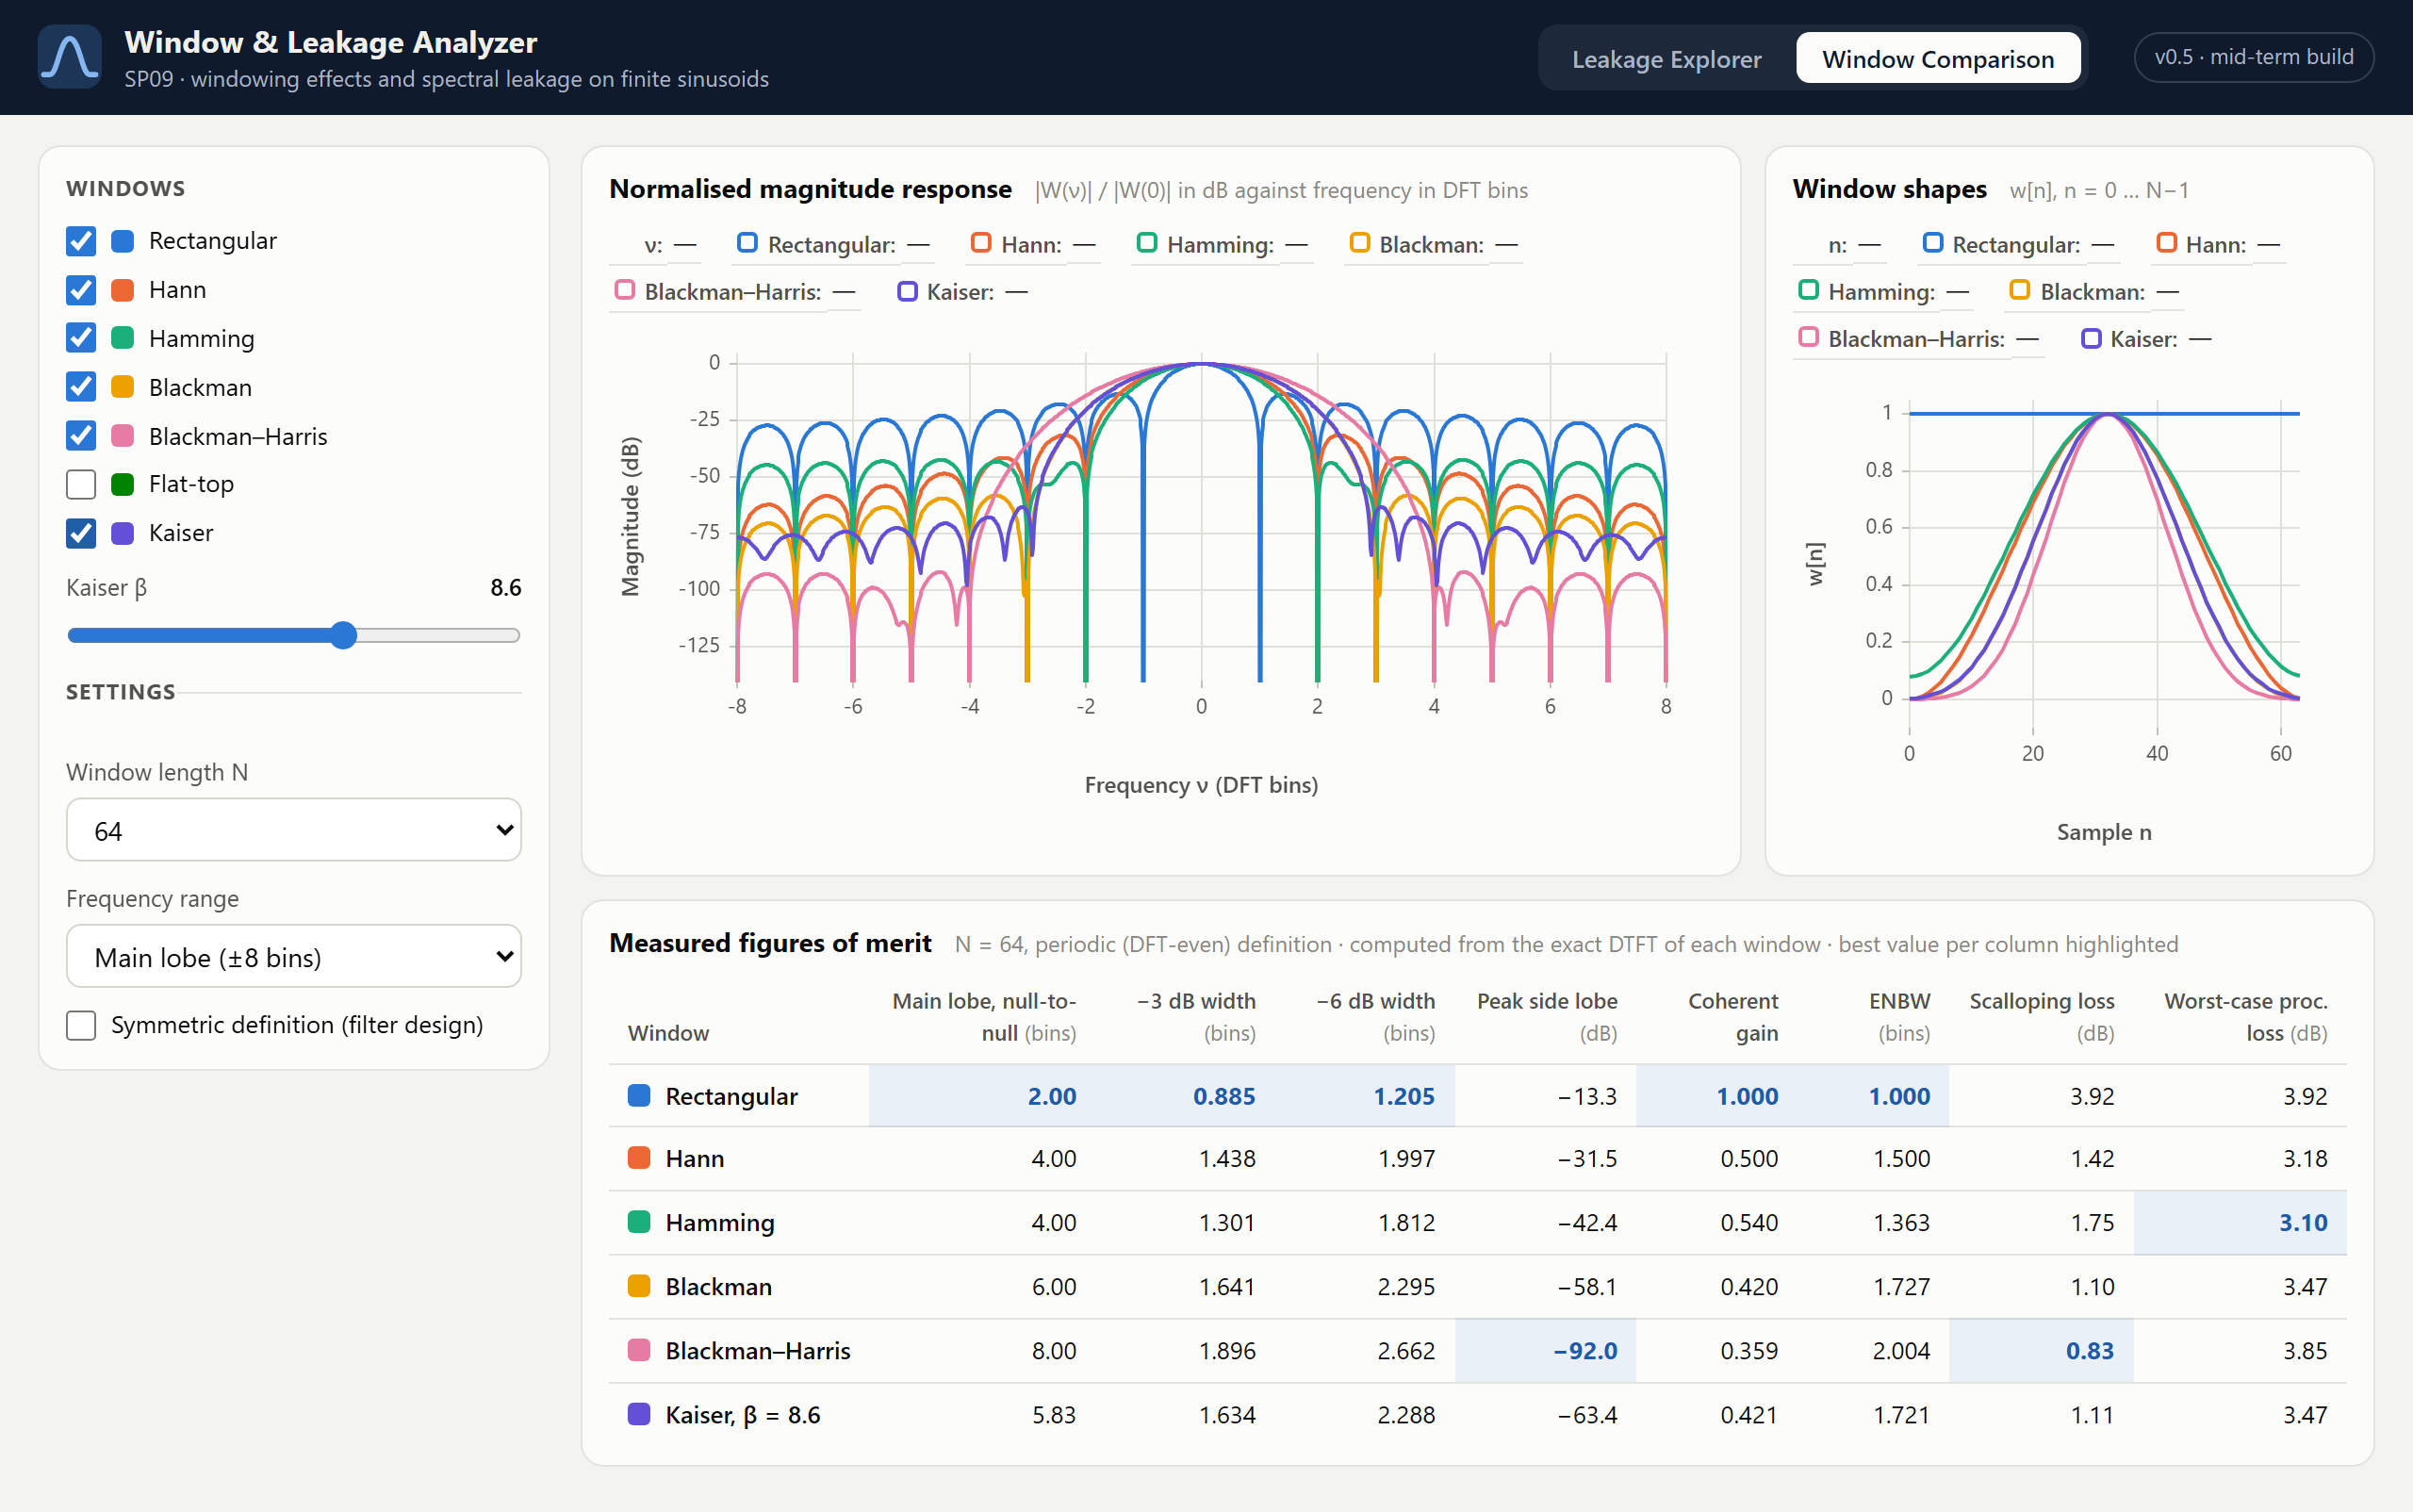
\includegraphics[width=\linewidth]{app_compare.png}
  \caption{Window Comparison view ($N=64$): normalised responses, window shapes and the
  measured figures of merit, with the best value in each column highlighted.}
  \label{fig:compare}
\end{figure}

\begin{table}[htbp]
  \centering\footnotesize
  \caption{Figures of merit measured by the app (periodic windows, $N=256$). CG: coherent gain;
  SL: scalloping loss; WCPL: worst-case processing loss.}
  \label{tab:metrics}
  \begin{tabular}{lrrrrrrrr}
\hline
Window & Null-to-null & $-3$\,dB & $-6$\,dB & PSL & CG & ENBW & SL & WCPL \\
 & (bins) & (bins) & (bins) & (dB) & & (bins) & (dB) & (dB) \\
\hline
Rectangular & 2.00 & 0.884 & 1.205 & $-$13.26 & 1.000 & 1.000 & 3.92 & 3.92 \\
Hann & 4.00 & 1.438 & 1.997 & $-$31.47 & 0.500 & 1.500 & 1.42 & 3.18 \\
Hamming & 4.00 & 1.301 & 1.812 & $-$42.66 & 0.540 & 1.363 & 1.75 & 3.10 \\
Blackman & 6.00 & 1.641 & 2.295 & $-$58.11 & 0.420 & 1.727 & 1.10 & 3.47 \\
Blackman--Harris & 8.00 & 1.896 & 2.662 & $-$92.01 & 0.359 & 2.004 & 0.83 & 3.85 \\
Flat-top & 10.00 & 3.721 & 4.578 & $-$92.75 & 0.216 & 3.770 & 0.01 & 5.77 \\
Kaiser ($\beta = 8.6$) & 5.83 & 1.634 & 2.288 & $-$63.26 & 0.421 & 1.721 & 1.11 & 3.47 \\
\hline
\end{tabular}

\end{table}

\begin{figure}[htbp]
  \centering
  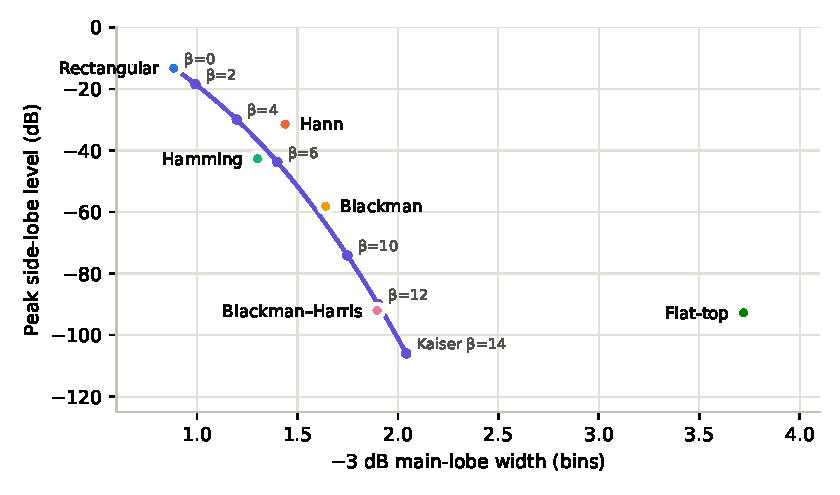
\includegraphics[width=0.78\linewidth]{tradeoff.pdf}
  \caption{Peak side-lobe level against $-3$\,dB main-lobe width, measured by the app ($N=256$).
  The Kaiser curve sweeps $\beta$ from 0 (rectangular) to 14.}
  \label{fig:tradeoff}
\end{figure}

\begin{figure}[htbp]
  \centering
  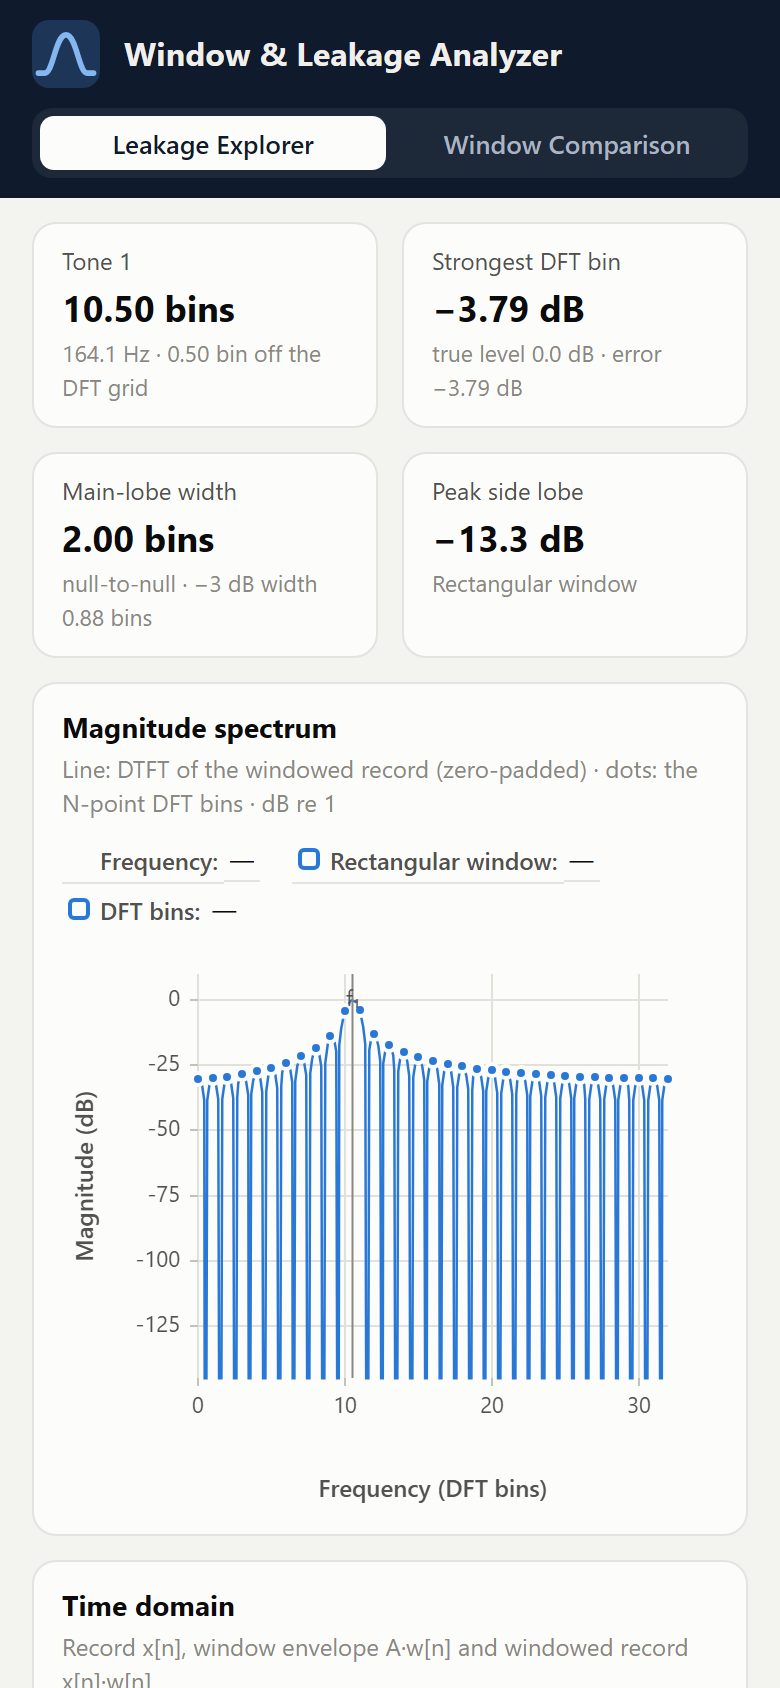
\includegraphics[width=0.3\linewidth]{app_phone.png}
  \caption{The same app on a 390-pixel-wide phone screen: plots first, controls below.}
  \label{fig:phone}
\end{figure}

\subsection{Validation results}
All 23 tests pass. Table~\ref{tab:validation} gives the largest disagreement with the
independent SciPy computation, taken over all seven windows. The widths agree to about
$10^{-8}$ bins and side-lobe levels to $2\times10^{-7}$\,dB. The Kaiser null differs by
$6\times10^{-5}$ bins, which is the grid resolution of the reference. Quantities with closed
forms agree to rounding error.

Comparing with the published Table~I of Harris (Table~\ref{tab:harris}) showed that some of its
entries differ from the exact values by more than its rounding:
\begin{itemize}
  \item Blackman $-3$/$-6$\,dB widths: 1.64/2.30 bins exactly, published as 1.68/2.35;
  \item Blackman--Harris $-6$\,dB width: 2.66 bins, published as 2.72;
  \item Hamming scalloping loss: 1.75\,dB, published as 1.78;
  \item Hann side-lobe level: $-31.5$\,dB, published as $-32$.
\end{itemize}
Our values agree with SciPy and with closed-form expressions, so the published entries appear to
be inaccurate. The tests therefore use closed forms rather than the table.

\begin{table}[htbp]
  \centering\small
  \caption{Largest $|\text{app}-\text{SciPy}|$ over the seven windows ($N=256$).}
  \label{tab:validation}
  \begin{tabular}{lrr}
\hline
Metric & Tolerance & Largest $|\text{app} - \text{SciPy}|$ \\
\hline
Main-lobe width, null-to-null (bins) & 1e-3 & 5.7e-5 \\
$-3$ dB width (bins) & 1e-3 & 4.7e-9 \\
$-6$ dB width (bins) & 1e-3 & 1.1e-8 \\
Peak side-lobe level (dB) & 1e-2 & 1.8e-7 \\
Coherent gain & 1e-9 & 5.6e-16 \\
ENBW (bins) & 1e-9 & 2.7e-15 \\
Scalloping loss (dB) & 1e-6 & 1.4e-14 \\
Worst-case processing loss (dB) & 1e-6 & 8.9e-15 \\
\hline
\end{tabular}

\end{table}

\begin{table}[htbp]
  \centering\footnotesize
  \caption{App value / value published in Harris~\cite{harris}, Table~I. Bold: differs by more
  than the table's rounding.}
  \label{tab:harris}
  \begin{tabular}{lrrrrrr}
\hline
Window & PSL (dB) & ENBW (bins) & $-3$\,dB (bins) & SL (dB) & WCPL (dB) & $-6$\,dB (bins) \\
\hline
Rectangular & $-$13.3 / $-$13 & 1.00 / 1.00 & 0.88 / 0.89 & 3.92 / 3.92 & 3.92 / 3.92 & 1.20 / 1.21 \\
Hann & \textbf{$-$31.5 / $-$32} & 1.50 / 1.50 & 1.44 / 1.44 & 1.42 / 1.42 & 3.18 / 3.18 & 2.00 / 2.00 \\
Hamming & $-$42.7 / $-$43 & 1.36 / 1.36 & 1.30 / 1.30 & \textbf{1.75 / 1.78} & 3.10 / 3.10 & 1.81 / 1.81 \\
Blackman & $-$58.1 / $-$58 & 1.73 / 1.73 & \textbf{1.64 / 1.68} & 1.10 / 1.10 & 3.47 / 3.47 & \textbf{2.30 / 2.35} \\
Blackman--Harris & $-$92.0 / $-$92 & 2.00 / 2.00 & 1.90 / 1.90 & 0.83 / 0.83 & 3.85 / 3.85 & \textbf{2.66 / 2.72} \\
\hline
\end{tabular}

\end{table}

% ------------------------------------------------------------------ 5
\section{Challenges and How They Were Addressed}
\begin{enumerate}[leftmargin=1.4em]
  \item \textbf{Reference values disagreed with our engine.} A unit test against the published
        Blackman $-3$\,dB width failed (1.641 vs 1.68 bins). Rather than adjust the code to fit,
        we derived the large-$N$ closed form and wrote an independent SciPy check. Both confirmed
        our value and revealed the other table discrepancies in Section~4.4. Since then the tests
        compare against closed forms, and SciPy is the external reference.
  \item \textbf{Measuring lobes precisely on a sampled spectrum.} Widths and side-lobe peaks read
        straight off an FFT depend on the amount of zero-padding. We use the FFT only to bracket
        each feature and then refine it on the exact DTFT, which makes the results independent of
        the grid (agreement with SciPy to $10^{-8}$ bins). Nulls must lie below $-20$\,dB, so
        pass-band ripple (as in flat-top windows) cannot be mistaken for a null.
  \item \textbf{Two definitions of the same window.} At small $N$, the symmetric and periodic
        forms give different figures of merit. For example, the ENBW of a Hann window at $N=64$ is
        1.524 bins in the symmetric form and 1.500 in the periodic form. The periodic form, used
        by Harris and SciPy, is the default, and the comparison view can switch definitions.
  \item \textbf{Stale plots during interaction.} Screenshot checks showed that dragging the
        frequency slider updated the read-outs but not the spectrum. The chart library skips
        its redraw when data is replaced without resetting the zoom. An explicit redraw fixed it,
        and slider events are now merged to one render per animation frame so dragging stays smooth.
  \item \textbf{Showing what cannot be plotted.} For an on-bin tone the DFT samples are exact
        zeros ($-\infty$\,dB), so the key ``single line'' picture was invisible. Those samples
        are now drawn at the bottom of the plot and labelled ``$\le -140$\,dB''.
  \item \textbf{Readability on phones.} At phone width the dense side-lobe pattern merged into a
        solid block. Thinner traces on small screens and a plots-first layout fixed this.
\end{enumerate}

% ------------------------------------------------------------------ 6
\section{Remaining Work and Timeline}
The second half finishes objectives O2, O4 and O6 and adds the analyses that need the
validated engine (Table~\ref{tab:plan}).

\begin{fixedtable}
  \small
  \caption{Plan for the second half (weeks counted from the mid-term review).}
  \label{tab:plan}
  \begin{tabularx}{\linewidth}{lY}
    \hline
    Week 1 & More windows: Bartlett, Tukey ($\alpha$), Gaussian ($\sigma$), Nuttall~\cite{nuttall} and
             Dolph--Chebyshev (equiripple); measure the side-lobe roll-off rate (dB/octave). \\
    Week 2 & Two-tone analyser: smallest resolvable separation, and whether a weak tone stays
             detectable, for each window and level difference; noise and SNR to illustrate ENBW. \\
    Week 3 & In-app trade-off charts (PSL vs width, ENBW vs scalloping); CSV/PNG export; shareable
             settings; built-in theory notes; dark mode; accessibility review. \\
    Week 4 & Progressive Web App with offline support; Android APK via Capacitor; iOS build
             (Capacitor on macOS, otherwise PWA install); testing on real devices. \\
    Week 5 & Public deployment (live link), automated tests on every push, feedback from classmates,
             performance check on low-end phones. \\
    Week 6 & Final report and demo video; buffer for fixes. \\
    \hline
  \end{tabularx}
\end{fixedtable}
The main risk is the iOS build, which needs macOS. The PWA route keeps the app usable on
iPhones either way.

% ------------------------------------------------------------------ references
\begin{thebibliography}{9}
  \bibitem{harris} F.~J. Harris, ``On the use of windows for harmonic analysis with the discrete
    Fourier transform,'' \emph{Proc.\ IEEE}, vol.~66, no.~1, pp.~51--83, Jan.~1978.
  \bibitem{oppenheim} A.~V. Oppenheim and R.~W. Schafer, \emph{Discrete-Time Signal Processing},
    3rd~ed. Pearson, 2010, chs.~7 and~10.
  \bibitem{kaiser} J.~F. Kaiser and R.~W. Schafer, ``On the use of the $I_0$-sinh window for
    spectrum analysis,'' \emph{IEEE Trans.\ Acoust., Speech, Signal Process.}, vol.~28, no.~1,
    pp.~105--107, Feb.~1980.
  \bibitem{nuttall} A.~H. Nuttall, ``Some windows with very good sidelobe behavior,''
    \emph{IEEE Trans.\ Acoust., Speech, Signal Process.}, vol.~29, no.~1, pp.~84--91, Feb.~1981.
  \bibitem{scipy} P.~Virtanen \emph{et al.}, ``SciPy 1.0: Fundamental algorithms for scientific
    computing in Python,'' \emph{Nature Methods}, vol.~17, pp.~261--272, 2020.
\end{thebibliography}

\end{document}
